% Etapes de conception, insister sur :
% architecture, choix, caractéristiques finales du système implanté

Nous allons présenter dans cette partie les principales étapes de conception
de notre réseau de neurones en détaillant tous les blocs réalisés et les choix
faits a propos de leur architecture.

\subsection{Programme de référence}
% Description du programme de référence en C, de l'utilisation de la base
% de données MNIST, du script en Python, des tableaux contenant les données,
% du taux d'erreur.
Le programme de référence implémente le même réseau de neurone que notre IP
mais directement en C. On peut ainsi l'executer sur un PC ou un micro-processeur 
et comparer les résultats avec l'implémentation réelle sur FPGA.

\subsubsection{L'algorithme}

\begin{algorithm}
	\SetAlgoLined
	\For {$f \leftarrow 0$ \KwTo $frames$} {
		$out1[neurons] \leftarrow 0$\;
		$out2[10] \leftarrow 0$\;
		\For {$r \leftarrow 0$ \KwTo $rows$} {
			\For {$c \leftarrow 0$ \KwTo $columns$} {
				\For {$n \leftarrow 0$ \KwTo $neurons$} {
					$out1[n] \leftarrow out1[n] + \texttt{get\_pixel(}f, r, j\texttt{)} \times w1[n][r][c]$\;
				}
			}
		}
		\For {$n \leftarrow 0$ \KwTo $neurons$} {
			$out1[n] \leftarrow \texttt{cut(}out1[n]\texttt{)}$\;
			$out1[n] \leftarrow out1[n] + b1[n]$\;
		}
		\For {$n \leftarrow 0$ \KwTo $neurons$} {
			\For {$i \leftarrow 0$ \KwTo $9$} {
				$out2[i] \leftarrow out2[i] + out1[n] \times w2[i][n]$\;
			}
		}
		\For {$i \leftarrow 0$ \KwTo $9$} {
			$out2[n] \leftarrow \texttt{cut(}out2[n]\texttt{)}$\;
			$out2[n] \leftarrow out2[n] + b2[n]$\;
		}
		$\texttt{assert(max(}out2\texttt{)} == \texttt{get\_label(}f\texttt{))}$\;
	}
	\caption{Boucle de calcul principal du réseau de neurone logiciel}
	\label{fig:soft_nn}
\end{algorithm}

L'algorithme~\ref{fig:soft_nn} page~\pageref{fig:soft_nn} implémente un réseau de neurones à deux étages.
Chaque étage réalise des multiplications et accumulations pour chaque pixel de
chaque image avec des poids, spécifiques à chaque neurone. Après chaque étage,
le résultat de chaque neurone est additionné avec une constante.

\subsubsection{Les données à traiter dans le réseau}

La configuration actuelle de ce réseau de neurone est adaptée pour la
reconnaissance de chiffres manuscrits de la base de données MNIST. Une image
en entrée ($28 \times 28$ pixels) correspond à un chiffre manuscrit de 0 à 9.
Le but de ce réseau de neurone est de reconnaître et d'identifier le chiffre
d'une image. Pour une image donnée, le chiffre identifié par le réseau correspond
au numéro du neurone de sortie qui a la plus grande valeur. \\
Dans ce modèle logiciel, les pixels sont encodés sur un octet, les poids et les
constantes sont sur 2 octets. Afin que dans le pire cas, aucune information ne
soit perdue lors de l'accumulation aux différents étages, on réalise cette opération sur
8 octets. Cependant, on ne doit en sélectionner que 2 sur les 8 pour effectuer l'ajout de la constante
sur des nombres de même taille et envoyer ce résultat au deuxième niveau. C'est
le rôle de la fonction \texttt{cut} qui permet de passer de 64 à 16 bits tout
en conservant le signe. Afin de choisir le bon masque, nous avons effectué
plusieurs essais et gardé celui qui menait au plus bas taux d'erreur (table
\ref{fig:masques} page~\pageref{fig:masques}).

\begin{table}[h!]
\centering
	\begin{tabular}{| l | l |}
	\hline
	Masque & Taux d'erreur \\ \hline
	0xFFFF0000 & 91.30 \\ \hline
	0x0FFFF000 & 91.30 \\ \hline
	0x03FFFC00 & 83.10 \\ \hline
	0x01FFFE00 & 28.80 \\ \hline
	0x00FFFF00 & 11.60 \\ \hline
	0x007FFF80 & 16.30 \\ \hline
	0x000FFFF0 & 90.70 \\ \hline
	\end{tabular}
	\caption{Essais de différents masques et leur taux d'erreur}
	\label{fig:masques}
\end{table}

Ainsi, nous masquons les résultats du premier niveau avec le masque sur 64 bits
\texttt{0x00FFFF00} (les bits de poids fort ne sont pas représentés ici) puis
nous effectuons un décalage pour garder uniquement ces bits, de 8 à 23. Ce
résultat nous a aussi aidé à effectuer le même masque et décalage dans notre
réseau de neurones matériel.

\subsubsection{Mise en forme des données MNIST}

Les poids des neurones et les constantes des étages de recodage
pour l'application MNIST, que nous utilisons dans
le logiciel de référence et dans notre IP nous ont été fournis au début du projet
sous forme de fichier texte où sont présentes toutes les données, séparées par
des virgules, et où chaque ligne correspond à un neurone. Un script Python nous
a permis d'analyser ces fichiers pour récupérer les données utiles et de les
replacer dans un unique fichier créé \texttt{net.c} avec les définitions de
4 tableaux d'entiers. Ce fichier est inclus et compilé dans le logiciel de référence et
pour le logiciel embarqué; ainsi les poids et les constantes sont
facilement accessibles depuis le logiciel. \\
Concernant les images, nous les avons récupérées à partir du site
officiel MNIST \linebreak (\texttt{yann.lecun.com/exdb/mnist/}) sous forme de fichiers
binaires où 1000 images de taille $28 \times 28$ pixels sont représentées comme
des tableaux d'octets en C. Un autre fichier binaire nous permet de connaître
le résultat, c'est-à-dire le digit, de chacune de ces images afin de comparer le
résultat de notre réseau de neurones avec le résultat attendu.
Les fonctions \texttt{get\_pixel} et \texttt{get\_label} permettent d'obtenir
facilement ces informations depuis le logiciel.

\subsubsection{Les résultats}

Les résultats du logiciel de référence en sortie de chacun des niveaux nous
sont utiles pour les comparer avec ceux de notre IP et s'assurer que les calculs
sont justes pour la classification des images MNIST. On s'attend à trouver
un même taux d'erreur minimal ($11.60\%$) car les configurations sont identiques
mais un calcul beaucoup plus rapide de toutes les images.

\subsection{IP du réseau de neurones}

\begin{figure}[h!]
	\begin{center}
		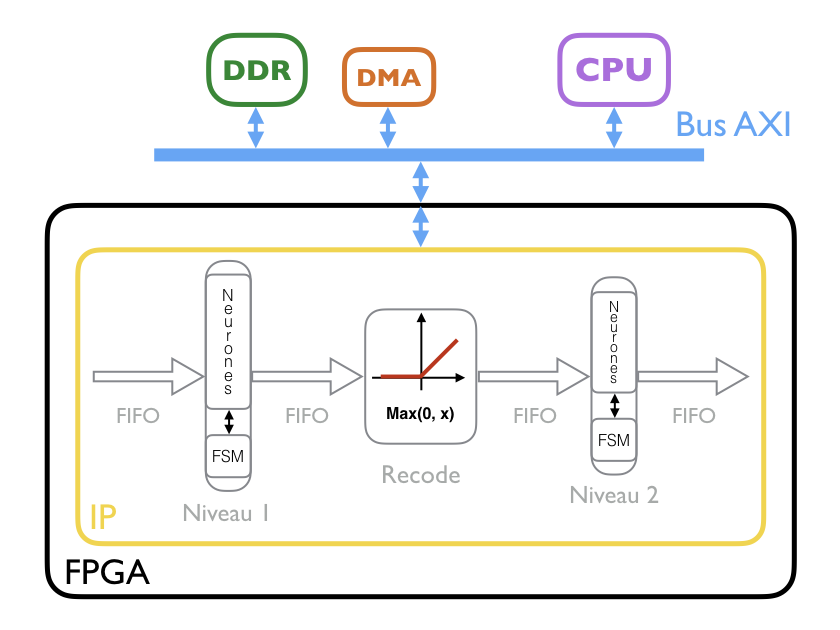
\includegraphics[scale=0.4]{NNSchema}
		\label{fig:NNSchema}
		\caption{Schéma de l'IP réseau de neurones dans son environnement }
	\end{center}
\end{figure}

\subsubsection{Le neurone}
	Le neurones est l'élément de base de notre réseau.
	C'est donc la première chose que nous avons implémenter.
	Pour faire cela, nous avons pensé le neurone en terme de
	fonctionnalités uniquement.
	Nous allons donc décrire ici la façons dont nous avons conçu un neurone. 
	Un neurones a deux modes de fonctionnement.
	Le premier est le mode de chargement des poids en mémoire, le second
	est le mode de calculs.

	\paragraph{Le mode de chargement des poids\\}
	
	Pour permettre aux neurones d'accomplir leur rôle principale, il faut que chaque neurone ai
	accès à leurs poids. Etant donné que chaque neurone doit disposer de ces propres poids
	(identiques pour une application donnée et donc pour une grandes quantité d'images)
	il est donc préférable que chaque neurone les mémorise. Afin d'accomplir cela,
	les neurones reçoivent une adresse (numero du poids à mémoriser) ainsi qu'un poids.
	Alors le neurones peut mémoriser le poids présent sur son entrée dans
	sa BRAM à l'adresse reçue à condition que ce neurones possède le {\em token} de
	configuration et qu'il reçoive le signal lui indiquant qu'un poids est présent sur son entrée.\\
	Le token de configuration est passé de neurones en neurones
	sur ordre du signal de contrôle pour qu'ils se configurent les uns après les autres.
	Vous trouverez une illustration de ce fonctionnement en
	figure~\ref{fig:N_poids} page~\pageref{fig:N_poids}.
	\begin{figure}[h!]
		\begin{center}
			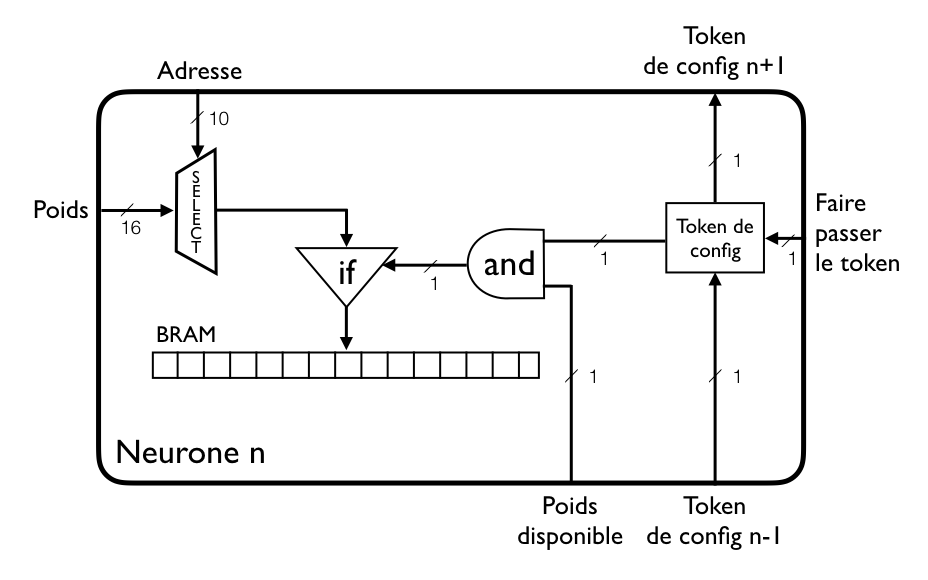
\includegraphics[scale=0.4]{N_poids}
			\caption{Schéma fonctionnel de l'implémentation du neurone en mode de configuration}
			\label{fig:N_poids}
		\end{center}
	\end{figure}

	\paragraph{Le mode de calcul\\}
	\begin{figure}[h!]
		\begin{center}
			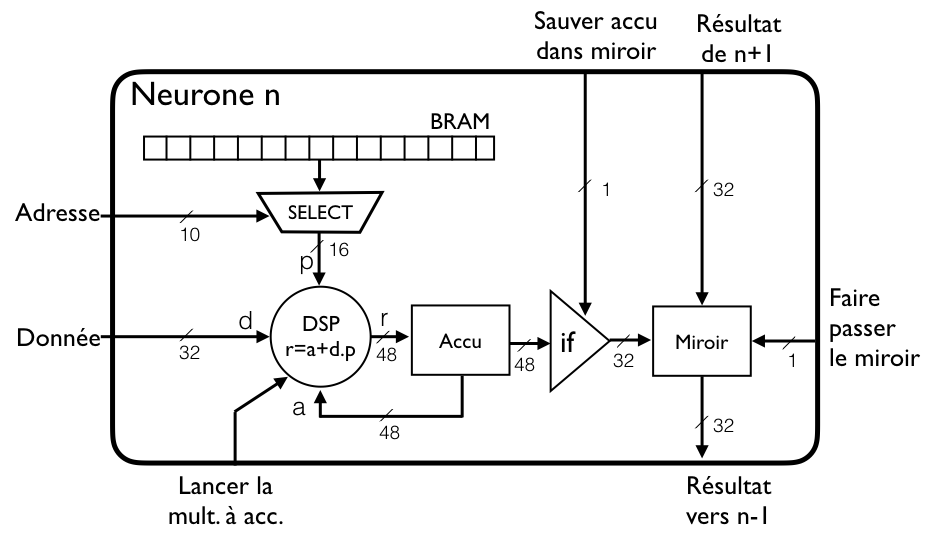
\includegraphics[scale=0.4]{N_calcul}
			\caption{Schéma fonctionnel de l'implémentation du neurone en mode de calcul}
			\label{fig:N_calcul}
		\end{center}
	\end{figure}
	
	Le mode de calcul est le mode principal d'un neurone. C'est dans ce mode que le neurone 
	reçoit des données et qu'il effectue une succession de multiplication à accumulation entre 
	la valeur du pixel reçu et le poids correspondant à l'adresse qui lui est donné. L'opération clé 
	d'un neurone peut être écrite comme :
	$$\sum_{adr=0}^n p_{adr}*d$$
	avec $n$ données entrantes dans le réseau, $p_{adr}$ le poids à l'adresse $adr$ 
	et $d$ la données entrante. 

	En effectuant cette opération sur chaque pixel d'une image, un neurone du premier niveau du réseau
	est capable de produire un résultat par image. Les neurones des niveaux suivant ne reçoivent 
	pas des pixels mais les résultats du niveaux précédent et opère de la même façon pour enfin 
	produire chacun un résultat (voir figure~\ref{fig:N_calcul} page~\pageref{fig:N_calcul}).
	\\{\em Notez qu'entre deux niveaux les résultats passent par l'étage de recode 
	(cf. Partie~\ref{plan:recode} "L'étage de recodage")}.
	
	Une fois que chaque neurone à produit son résultat, ils vont en faire une copie dans 
	un registre appelé {\em miroir} (au signal de {\em faire copie de accu dans miroir}) 
	et remettre le registre d'accumulation à 0. Ainsi, le calcul de l'image suivante pourra 
	être commencé alors que résultat de l'image précédente 
	sera évacué vers la FIFO de sortie suivante. Pour ce faire, à la réception du signal 
	{\em faire passer le miroir}, chaque neurones va faire passer la valeur de son 
	registre miroir au neurone suivant et récupérer la valeur du miroir du neurone précédant.
	Cela permet de ne connecter qu'un neurone à la FIFO de sortie 
	et de faire évacuer les données les unes après les autres dans cette FIFO 
	(voir figure~\ref{fig:N_calcul} page~\pageref{fig:N_calcul}).
	
\subsubsection{La machine à états (FSM) du niveau de neurones}

\subsubsection{Le niveau de neurones}
%TODO: Hugues
\subsubsection{L'étage de recodage}
\label{plan:recode}

\subsection{Logiciel de commande}
Le logiciel de commande est le logiciel embarqué sur la carte, qui s'execute
sur processeur ARM. Celui ci permet de configurer notre réseau de neurones avec
les poids et les constantes choisies, de lancer les calculs avec les valeurs
voulues et de récupérer les résultats. Il s'écrit en C et s'interface avec
l'utilisateur grâce à la liaison série (composant UART). Le squelette de base
était déjà disponible avec toutes les fonctions nécessaires, le code était
écrit pour la configuration d'un niveau de neurone, l'envoi d'images simples et
la récupération des résultats. Les données
concernant les poids, les constantes, les images et les paramètres (taille d'une
image, nombre de neurones à chaque niveau, nombre d'images) étaient toutes notées
dans un fichier (\texttt{dataset.h}). Nous avons gardé ce fonctionnement pour la
majeur partie de notre projet car il nous a permis de tester facilement notre
IP pour des images de petites tailles, des niveaux de neurones avec très peu
de neurones (3) et de configurer facilement les pixels des images et les poids
choisis pour connaître les résultats attendus et comparer avec ceux de notre IP.
Nous avons cependant complété ce code afin qu'il puisse gérer notre IP complète
avec deux niveaux de neurones et un étage de recodage.
Par la suite, nous avons repris les mêmes données MNIST que pour le logiciel de
référence afin de tester l'application réelle. \\

\subsubsection{Moyens de communication avec l'IP}
Pour pouvoir échanger des données entre le logiciel embarqué et notre IP, 16
registres de 32 bits peuvent être lus et écrits des deux côtés de notre
système. Par exemple
les 4 premiers bits de registre 3 contiennent la configuration actuelle de notre
IP : mode envoi des images, mode configuration (cad chargement des poids) du
niveau 1, 2 ou de l'étage de recodage. Cette configuration est transmise
aux blocs concernés afin qu'ils changent leur comportement et attendent les
données utiles en entrée. Un autre bit de ce registre permet de d'envoyer le
signal \texttt{RESET} à toute notre IP.
Les registres sont accédés avec un offset à partir d'une adresse de base
sur le bus AXI. Des fonctions utilitaires déjà présentes
permettent de faciliter les accès grâce à des masques et des opérations
binaires avec les bons registres. \\
Pour envoyer ou recevoir de plus grosses quantités de données comme l'envoi
des poids ou des frames, ou récolter les résultats de notre réseau de neurones,
on utilise la fonction burst de notre bus AXI. On peut alors transférer des
données de façon rapide entre la DDR où le logiciel alloue de l'espace
pour stocker poids, frames et résultats et les FIFOs d'entrée et de sortie pour
communiquer avec notre réseau de neurones. \\
A chaque fois que l'on souhaite faire un transfert, les mêmes opérations sont
faites :
\begin{itemize}
	\item si c'est une écriture, les données à écrire sont présentes, comme
		variables globales, dans des tableaux multi-dimensions dans un
		fichier C
	\item on alloue un tableau d'entiers (signé pour les poids, non signé
		pour les frames) de 32 bits de manière dynamique. La taille
		du tableau alloué dépend des données considérées mais on alloue
		32 bits (1 case du tableau) par donnée (1 poids, 1 constante ou
		1 pixel d'une frame) afin de faciliter leur traitement par l'IP,
		les FIFOs ayant des cases de même taille.
	\item afin de préparer ce tableau aux bursts, qui sont des transferts
		par bloc
		de 16 mots de 32 bits, soit 16 cases du tableau vers une FIFO,
		on doit aligner son adresse sur des frontières de $16 \times
		4$ octets. On ajoute alors $16 \times 4$ comme supplément à la
		taille nécessaire du tableau et on incrémente l'adresse
		renvoyée par \texttt{malloc} jusqu'à trouver une frontière de
		$16 \times 4$ octets, cad une adresse terminant par
		\texttt{0x00}, \texttt{0x40}, \texttt{0x80} ou \texttt{0xC0}.
		Grâce au supplément dans la taille ajouté, on est sûr d'avoir
		suffisament de place pour écrire les données même après avoir
		incrémenté l'adresse pour l'arrondir.
	\item on écrit les données dans le tableau alloué à partir des
		variables globales déjà présentes
	\item on passe l'adresse de ce tableau à l'IP par un registre
	\item on indique dans un autre registre le nombre de bursts nécessaires
		pour transférer tout le tableau vers la FIFO. Si le tableau n'a
		pas un nombre de case qui est multiple de 16, on fait un burst
		supplémentaire pour inclure le reste. Il faudra alors
		envoyer à l'IP un signal \texttt{RESET} entre deux écritures
		afin de vider les FIFOs de leurs données résiduelles invalides.
\end{itemize}
% TODO: inclure schéma général qui résume ces transactions
\subsubsection{Débogage}
% problèmes uniquement liés au soft : printf et GDB
% (allocation et remplissage des tableaux)
Pour déboguer le système global, notre IP avec le logiciel embarqué nous avons
utilisé différentes manières. \\
Pour des problèmes uniquement liés au logiciel (mauvaise taille, mauvais indices
des tableaux, ...),
nous avons utilisé le composant
UART avec la fonction Xilinx \texttt{printf} pour envoyer par le lien série des
informations sur un terminal distant. En passant par la suite à la carte ZedBoard,
nous avons pu faire fonctionner la fonction Debug sur SDK Xilinx pour pouvoir
avancer pas à pas dans le code et inspecter l'état des variables. \\
% problèmes de l'IP :
% informations contenues dans certains registres
Les problèmes liés à notre IP sont plus difficiles à déboguer car nous ne pouvons
pas simuler le système complet à cause de licences manquantes. Pour repérer
certains problèmes comme des boucles d'attente infinies, des données de
notre IP sont écrites dans des registres comme les signaux \texttt{READY} et
\texttt{ACK} de chacunes des FIFOs et les \texttt{COUNT} pour ces FIFOs. Des
fonctions utilitaires permettent de lire facilement ces informations à partir
des registres concernés et de nous renseigner plus précisément sur quel est
l'étage bloquant de notre système. \\
% fonctions pour poper des valeurs en cours de route
Cependant ces méthodes ne peuvent nous renseigner uniquement sur l'étage qui
fait bloquer tout le système et non pas sur la validité des données produites
en sortie de chaque étage.

\subsection{Caractéristiques finales du système implanté}
% Donner ici les performances du système ?
% Comparer avec le logiciel de référence
% Comparer avec, en théorie, les performances maximales que l'on pourrait
% avoir en HW

